\chapter{Implementation, Runtime Behaviour, and Operations}
\thispagestyle{plain}
\section*{Introduction}
\addcontentsline{toc}{section}{Introduction}
This chapter explains how the architecture executes in practice. It covers the shared backend skeleton, the runtime startup sequence, database and cache usage, asynchronous workflows, AI-assisted analysis paths, deployment mechanics, observability, resilience, performance characteristics, and representative features exposed through the user interface.

\section{Implementation Philosophy}
Implementation choices in this project were not made solely for code elegance. They were driven by a recurring tension between correctness, latency, operability, and dependency fragility. A useful way to read the implementation is therefore to distinguish essential complexity from accidental complexity. Essential complexity comes from the problem domain itself: many feeds, many entity types, partial failure, context-sensitive prioritization, and AI-assisted summarization. Accidental complexity comes from avoidable inconsistency, duplicate infrastructure logic, ad hoc configuration, and uncontrolled side effects.

Much of the repository's engineering discipline is aimed at reducing accidental complexity. Shared factories, shared libraries, uniform transaction boundaries, and explicit startup hooks do not make the domain simpler, but they do make the codebase more predictable. That predictability is academically relevant because it is one of the main preconditions for maintainability in a multi-service system.

\section{The Shared Backend Skeleton}
The most important implementation pattern in the repository is that all services share one application factory. The factory sets up structured logging, correlation IDs, health checks, and error handling; each service then adds its own routers and startup hooks.

\begin{lstlisting}[caption={Shared service factory excerpt},label={lst:factory-new}]
def create_service_app(*, settings, title, description="",
                       on_startup=None, on_shutdown=None):
    configure_logging(settings.service_name, settings.log_level)
    app = FastAPI(title=title, version="0.1.0", lifespan=lifespan)
    app.add_middleware(CorrelationIdMiddleware)
    register_error_handlers(app)
    @app.get("/health")
    async def health():
        return {"status": "ok", "service": settings.service_name}
    return app
\end{lstlisting}

The omission is as important as the inclusion: JWT middleware is not wired in the factory because key retrieval happens during startup. This small decision prevents premature configuration coupling between service import time and runtime secret availability.

The broader implementation lesson is that lifecycle order matters. In distributed applications, it is often incorrect to assume that everything required by request-time logic is already available at import time. The repository explicitly models startup as a separate phase in which secrets, keys, pools, caches, and clients are acquired. This yields a more accurate program structure than pretending initialization and steady-state request handling are the same kind of work.

\section{Startup Lifecycle and Runtime State}
The per-service startup flow follows a repeatable pattern: initialize the async SQLAlchemy engine, create or obtain a session factory, attach a Redis cache if the service uses one, construct a secrets client when startup secrets are required, build AI clients only in services that need them, create source-health repositories only in services that talk to external sources, then wire auth bootstrap.

Figures~\ref{fig:runtime-flow-new} and \ref{fig:runtime-flow-bottom} summarize the sequence.

\begin{figure}[H]
\centering
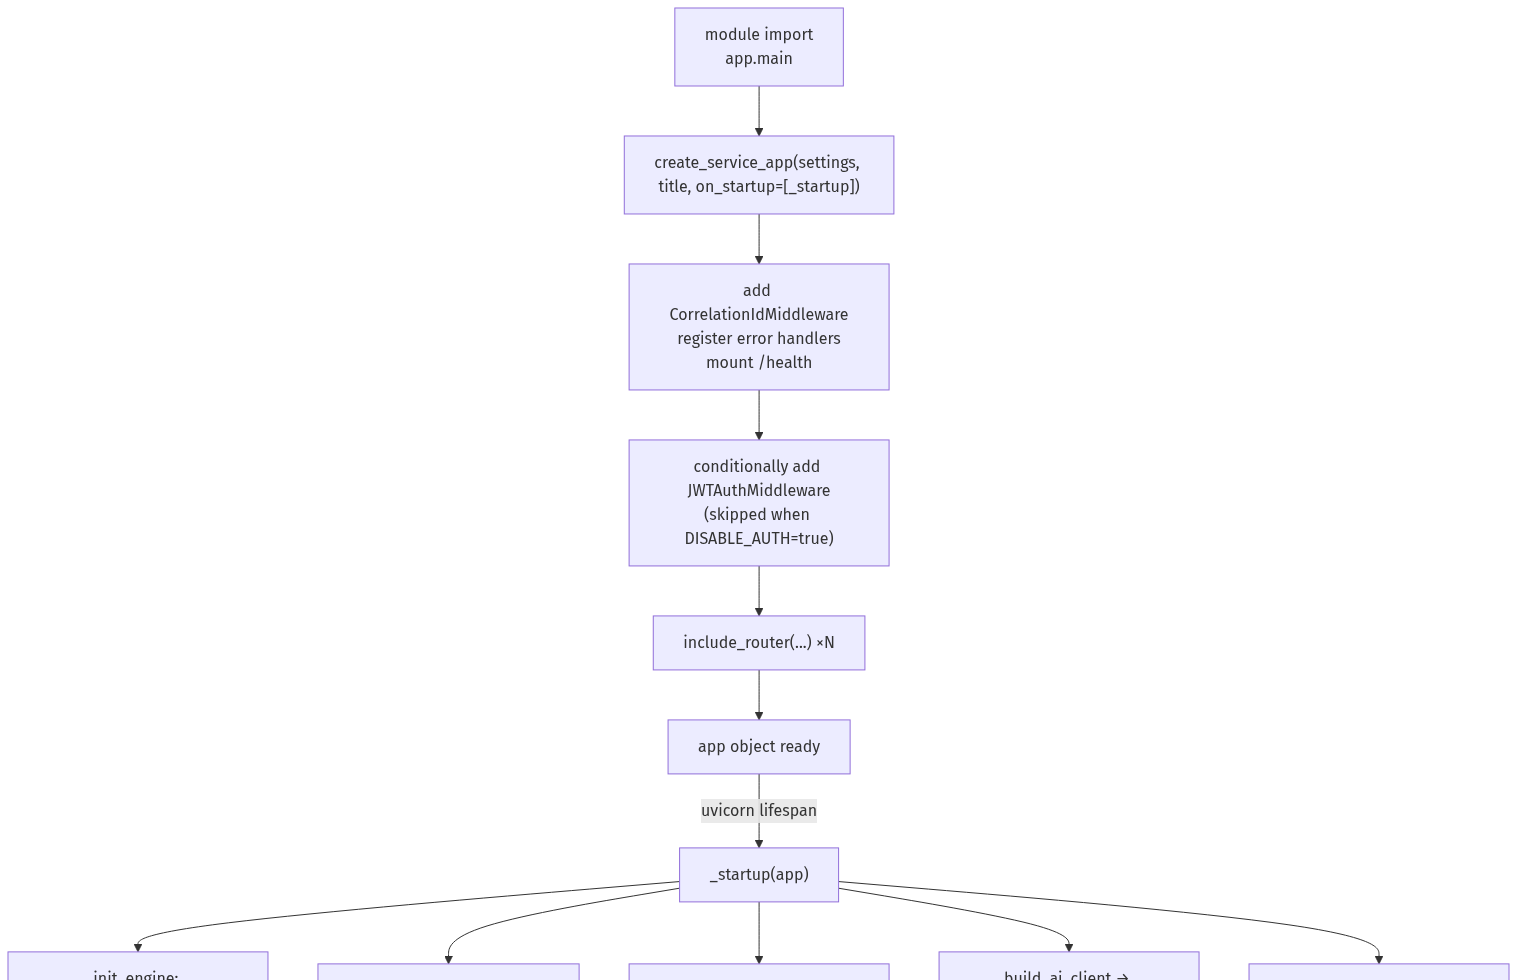
\includegraphics[width=0.92\textwidth]{images/tip/diagrams/10_runtime_flow_top.png}
\caption{Service runtime flow from startup hooks to request handling, upper segment.}
\label{fig:runtime-flow-new}
\end{figure}

\begin{figure}[H]
\centering
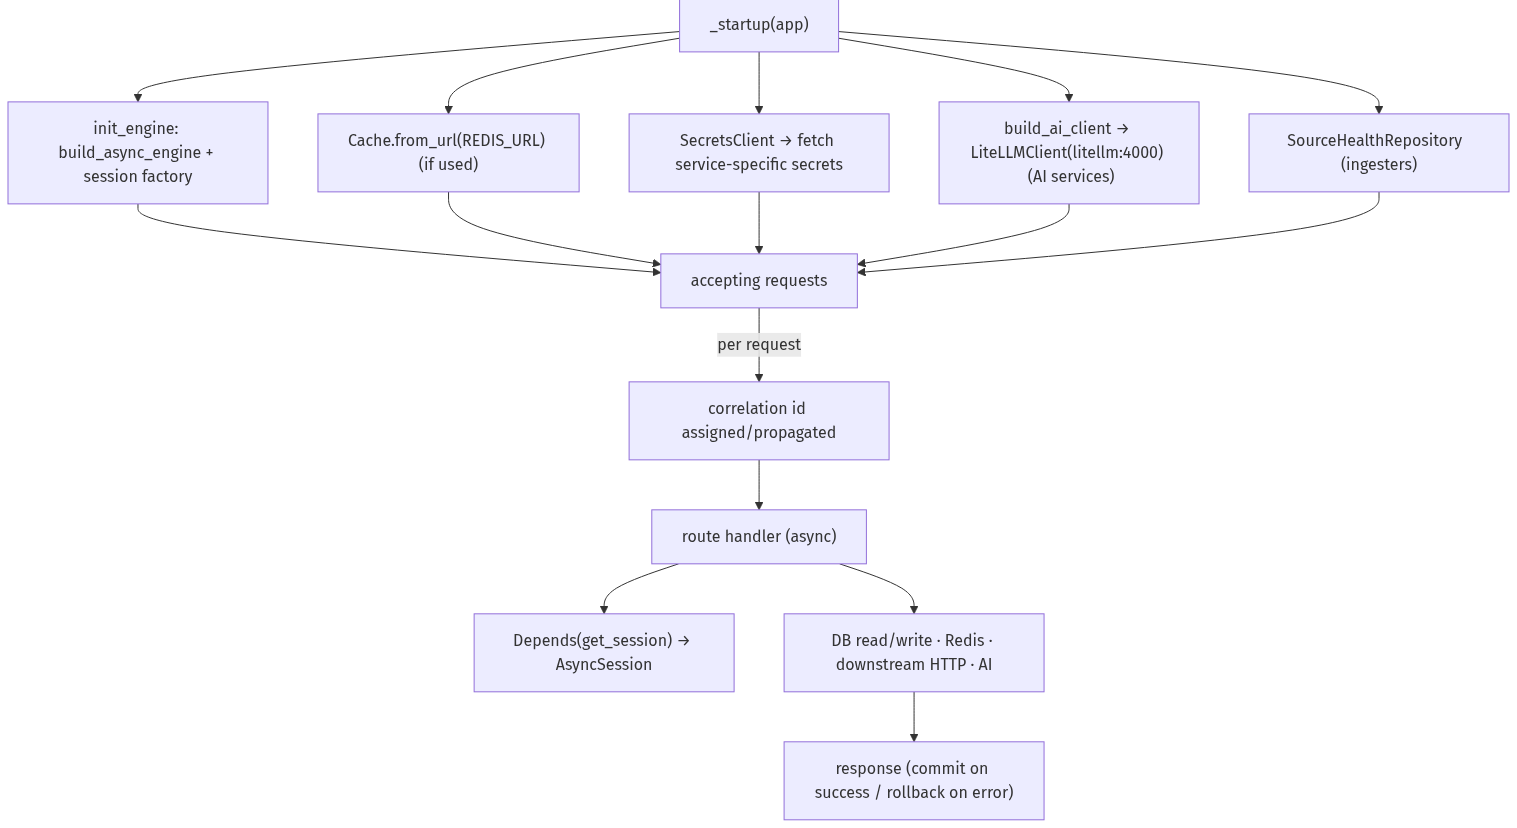
\includegraphics[width=0.92\textwidth]{images/tip/diagrams/10_runtime_flow_bottom.png}
\caption{Service runtime flow from startup hooks to request handling, lower segment.}
\label{fig:runtime-flow-bottom}
\end{figure}

This pattern offers a useful compromise. Shared operational concerns are centralized, but runtime capability remains opt-in. A simple CRUD-style service does not carry the cost of the full AI stack, while an ingest service can attach health tracking and resilient HTTP without duplicating infrastructure code.

From a software design perspective, this is a form of capability-based composition. A service acquires only the runtime components needed for its actual role. This reduces unnecessary transitive complexity and limits the number of active failure paths in simpler services. It also makes the service graph easier to reason about because optional capabilities are visible during startup rather than hidden in always-on global state.

\section{Database Access and Transaction Boundaries}
Database access is implemented with async SQLAlchemy sessions wrapped in a dependency that commits on success and rolls back on failure.

\begin{lstlisting}[caption={Per-request transaction boundary},label={lst:session-new}]
async def get_session(factory):
    async with factory() as session:
        try:
            yield session
            await session.commit()
        except Exception:
            await session.rollback()
            raise
\end{lstlisting}

This implementation has two notable consequences. First, route handlers stay focused on domain logic rather than transaction management. Second, service-wide behaviour is consistent, which matters in a multi-service monorepo where inconsistent transaction boundaries would be difficult to reason about.

There is also an important correctness property here. By placing commit and rollback responsibility in one shared dependency, the repository reduces the risk of partially applied request logic caused by handler-local transaction management. In practical terms, this means the developer is less likely to forget to commit, over-commit, or leak transaction scope across unrelated operations.

\section{Resilient Outbound Communication}
Every external call is assumed to be fallible. The shared resilience layer provides retry policy, retryability rules, timeout handling, and circuit-state integration with source health. The retry policy itself is intentionally modest: three attempts, exponential backoff, and jitter.

\begin{lstlisting}[caption={Retry policy for external source calls},label={lst:retry-new}]
@dataclass
class RetryPolicy:
    max_attempts: int = 3
    base_delay: float = 1.0
    backoff: float = 2.0
    jitter: float = 0.25
\end{lstlisting}

The architecture treats partial success as normal. Ingestion tasks gather concurrent source calls and record source-level failures rather than aborting the entire cycle on the first upstream error. This is one of the clearest examples of the repository's availability-first design philosophy.

This also illustrates a fundamental distributed-systems idea: failure is not exceptional at system scale. It is expected. The role of implementation patterns such as retries, backoff, and circuit state is not to create the illusion of perfect reliability. It is to shape how failure manifests, to keep it bounded, visible, and recoverable.

\section{Asynchronous Workflows and Scheduler Semantics}
The platform uses asynchronous execution in three distinct ways.

\subsection{Concurrent I/O Fan-Out}
Independent upstream calls are executed concurrently with \texttt{asyncio.gather}. This is used both in ingestion cycles and in multi-source investigative workflows.

\subsection{Background Task Continuation}
Long-running operations return quickly and complete in the background. The orchestrator's analysis cycle and some vulnerability backfill paths use this pattern so that endpoints can acknowledge work without holding an HTTP request open unnecessarily.

\subsection{Scheduler Callback Completion}
Scheduler-triggered jobs use a run identifier so asynchronous tasks can call back into the scheduler when they actually finish. This is an important implementation refinement: it prevents the scheduler from treating \texttt{202 Accepted} as implicit success. The platform therefore records long-running jobs as \texttt{running} until the callback arrives or the watchdog times them out.

Figure~\ref{fig:async-new} captures these execution patterns.

\begin{figure}[H]
\centering
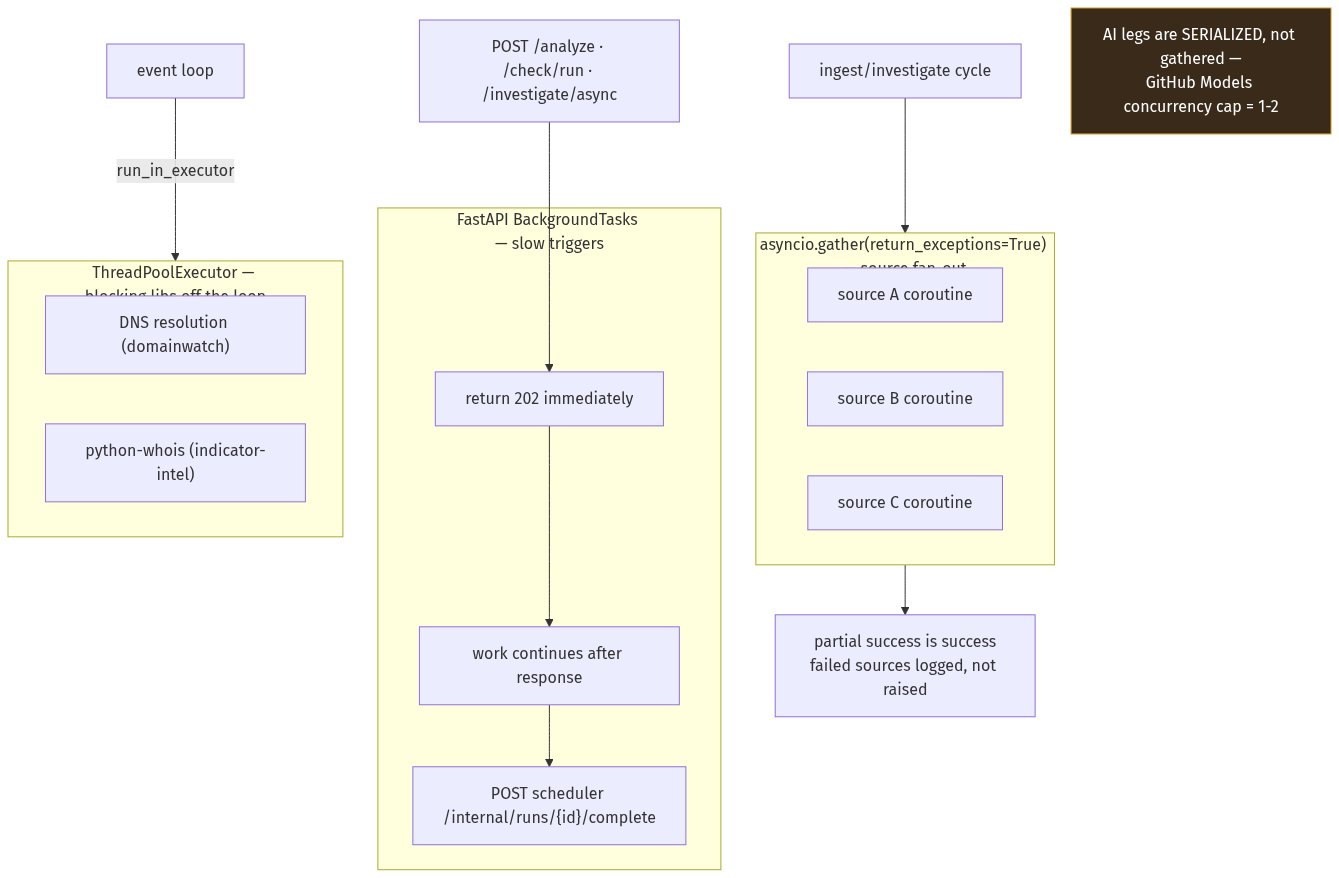
\includegraphics[width=0.92\textwidth]{images/tip/diagrams/10_async_execution.png}
\caption{Asynchronous execution patterns in the platform.}
\label{fig:async-new}
\end{figure}

\section{AI-Assisted Security Workflows}
AI is integrated into the platform as a bounded analytical layer rather than as a universal dependency.

This boundary is central to the implementation's soundness. AI systems are high-variance dependencies: they can fail, drift, hallucinate, or hit quota limits independently of the rest of the application. Treating them as ordinary synchronous business-logic calls would therefore contaminate ingestion, CRUD paths, and operator workflows with unnecessary volatility. By isolating AI behind a gateway and keeping it off the ingestion hot path, the implementation converts an unreliable external capability into a contained optional subsystem.

\subsection{Gatewayed AI Access}
All AI-capable services talk to a LiteLLM proxy instead of holding provider-specific credentials directly. This centralizes provider keys, creates one auditable outbound AI surface, and makes fallback routing a proxy concern rather than a per-service concern.

\subsection{Typed Structured Outputs}
AI calls that are expected to produce machine-usable results are validated against Pydantic schemas. This is one of the most technically mature aspects of the implementation. Instead of trusting a free-form string, the platform requests JSON-compatible outputs, validates them, and retries once on validation failure. The result is that orchestration code deals with typed objects rather than brittle prompt text.

The theoretical significance of this choice is larger than it first appears. It is an example of interface hardening. Instead of allowing a probabilistic model to define its own output format on each call, the application constrains the interaction contract. This reduces downstream ambiguity and makes it possible to distinguish three different failure classes clearly: provider failure, invalid structure, and semantically weak but structurally valid content. Only the last class still requires human review, which is exactly where it belongs.

\subsection{The Orchestrator Analysis Cycle}
The orchestrator performs a four-step cycle over already-ingested data: CVE relevance ranking, actor likelihood ranking, detection correlation, and executive briefing. A separate geo-prediction job runs on its own cadence. Each step persists outputs independently, which means one late-stage failure does not discard earlier successful analysis. This is a sound operational decision for quota-limited and failure-prone external model dependencies.

\subsection{Deep Indicator Investigation}
The indicator-intel service performs a more forensic-style workflow. It gathers context from passive and locally stored sources, performs dorking and enrichment, and returns a synthesized view rather than a single-source verdict. The feature is slower than the hot lookup path by design and is therefore architecturally separated from it.

This separation is conceptually important because it acknowledges two different temporal modes of security work. Triage requires speed and bounded latency. Investigation requires breadth and tolerates more delay in exchange for richer context. Trying to satisfy both with one endpoint often produces a poor compromise. The repository instead implements a dual-path design: a fast verdict path and a deeper enrichment path.

\section{Representative Features and Their Realization}
\subsection{The Dashboard}
The dashboard is not a static page backed by one service. It is powered by a frontend aggregation route that fans out to multiple backend services in parallel, then reshapes the result into one UI-oriented payload. This is a good use of the BFF pattern because it keeps composition logic close to the interface without forcing backend services to expose dashboard-specific payloads.

\begin{figure}[H]
\centering
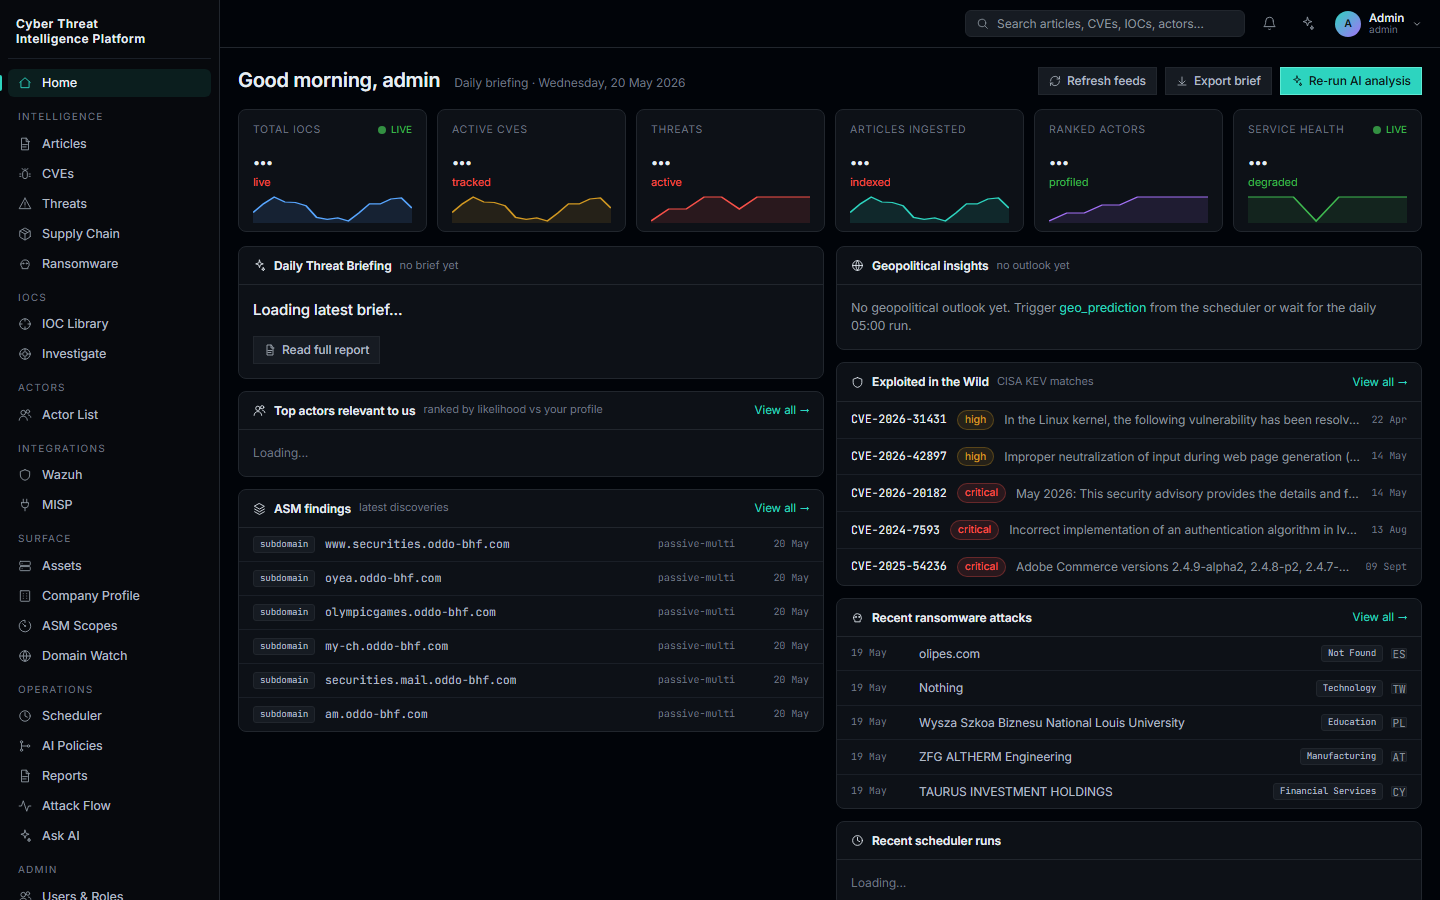
\includegraphics[width=0.95\textwidth]{images/tip/shots/02_dashboard.png}
\caption{Dashboard view assembled through the frontend aggregation route.}
\label{fig:dashboard-new}
\end{figure}

\subsection{IOC Lookup and Investigation}
The platform deliberately distinguishes between a sub-second lookup path and a slower investigation path. The first is optimized for triage and cache locality. The second is optimized for contextual depth.

\begin{figure}[H]
\centering
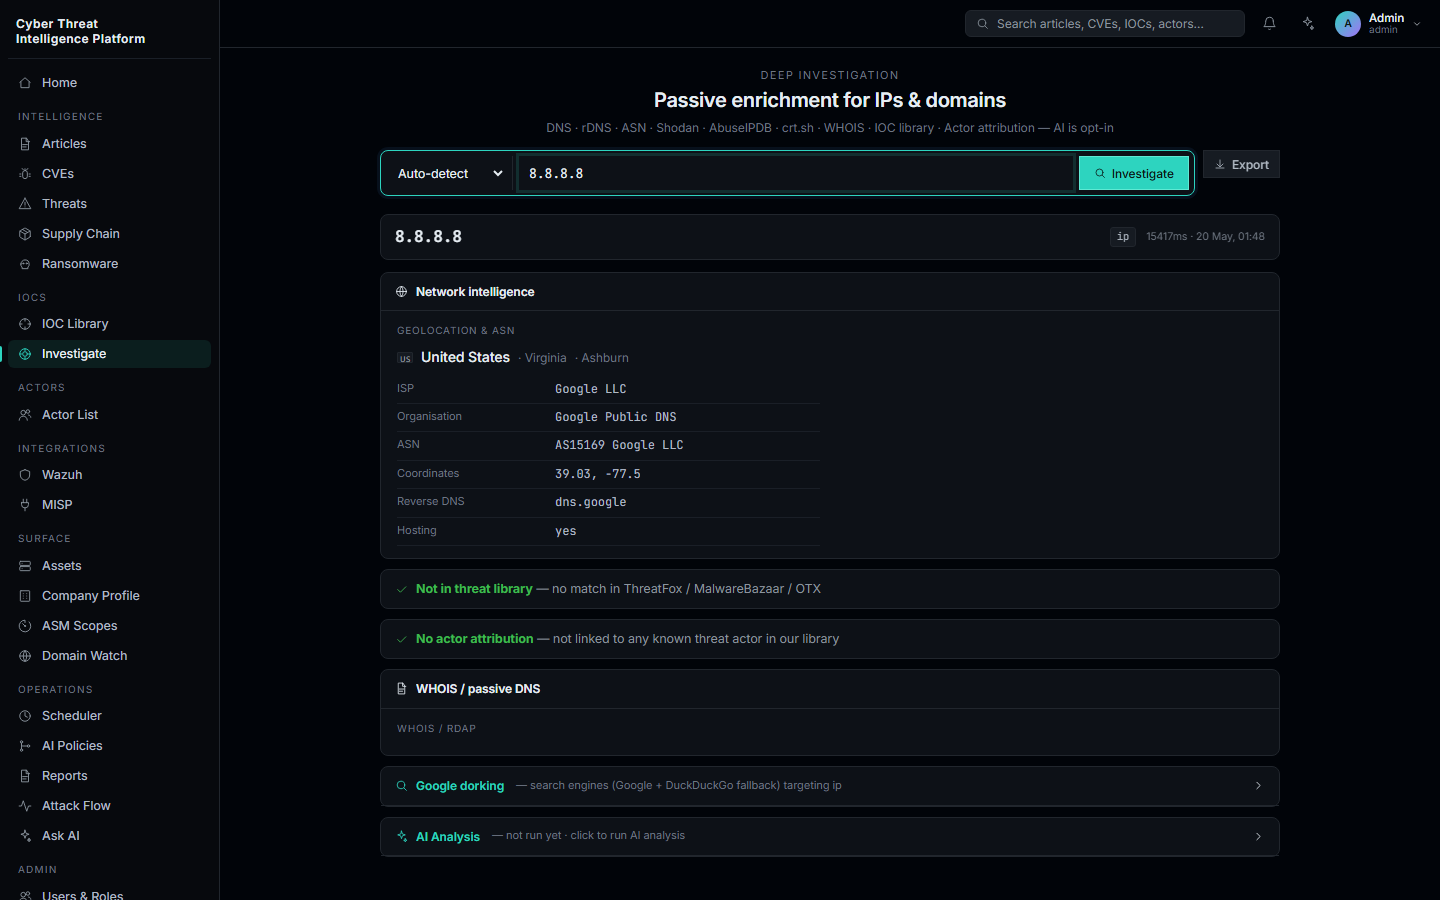
\includegraphics[width=0.95\textwidth]{images/tip/shots/16_ioc_investigate_result.png}
\caption{Indicator investigation result with multi-source enrichment.}
\label{fig:ioc-investigate-new}
\end{figure}

\subsection{Asset and Profile Context}
The CMDB service stores both assets and the company profile used by downstream synthesis. This is architecturally significant because it means vulnerability prioritization and actor ranking are not purely generic; they are conditioned on the organization's declared technologies, sectors, geographies, and threat concerns.

\begin{figure}[H]
\centering
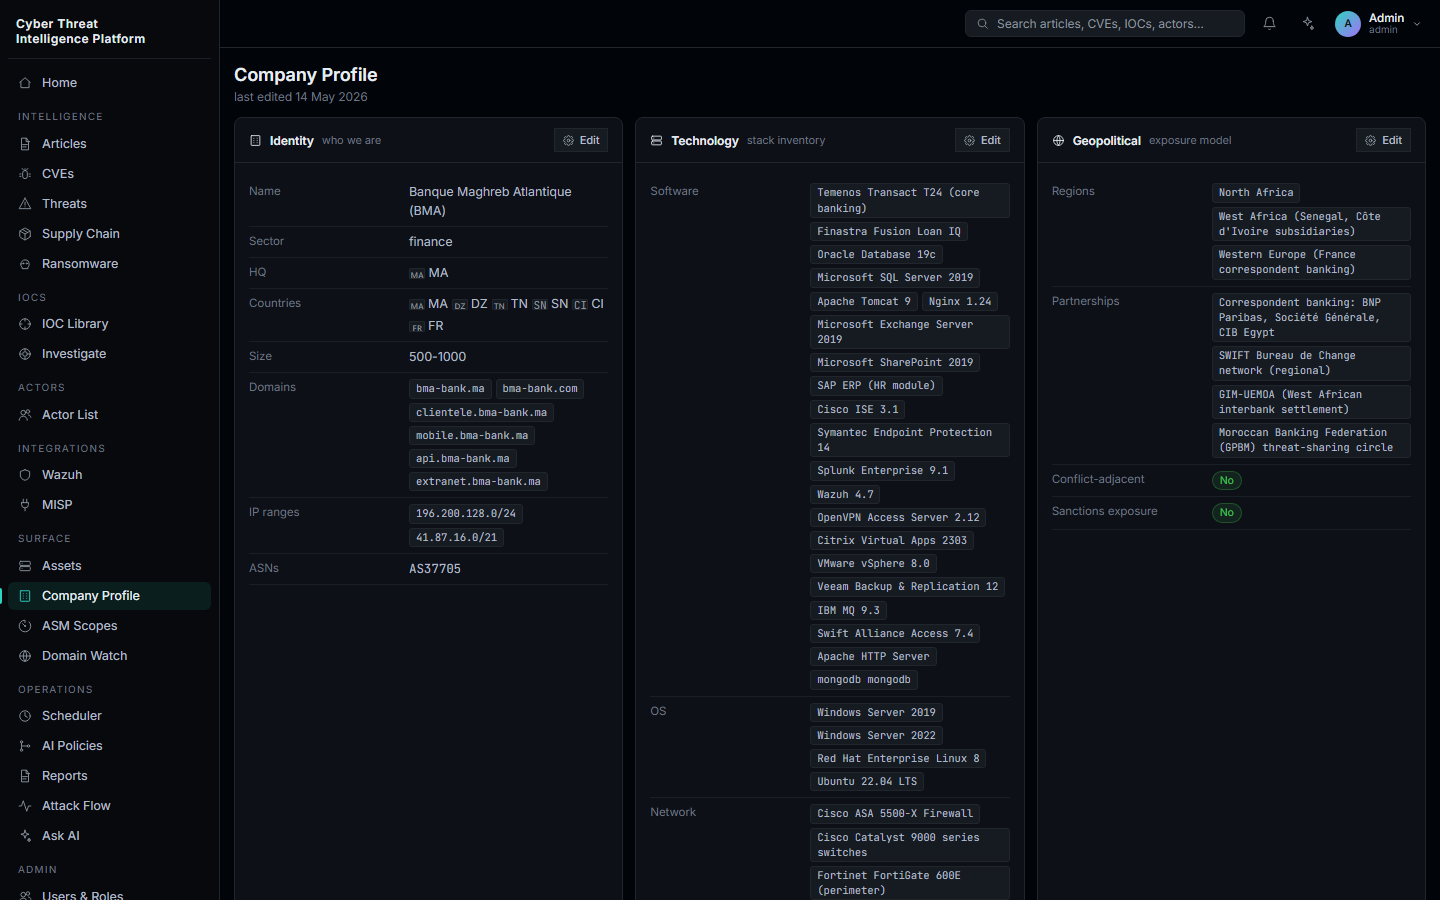
\includegraphics[width=0.95\textwidth]{images/tip/shots/23_assets_company_profile.png}
\caption{Company profile management in CMDB.}
\label{fig:company-profile-new}
\end{figure}

\subsection{Reports, Policies, and Flow Visualization}
Reports, AI policies, and generated attack flows give the system a managerial and analytical surface beyond simple list views.

\begin{figure}[H]
\centering
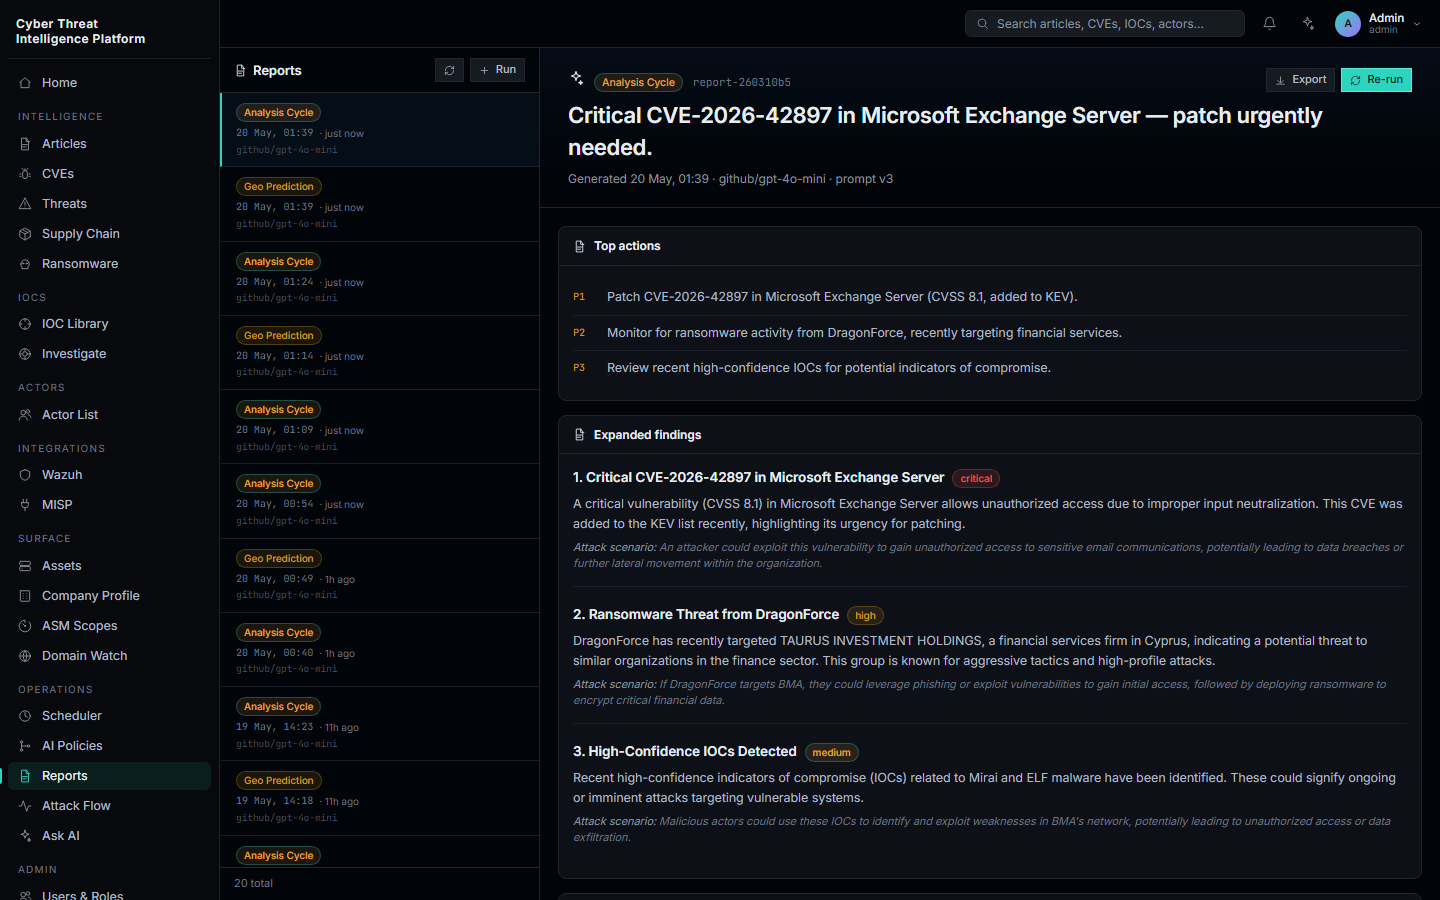
\includegraphics[width=0.95\textwidth]{images/tip/shots/31_reports.png}
\caption{Persisted report outputs generated by the orchestrator.}
\label{fig:reports-new}
\end{figure}

\begin{figure}[H]
\centering
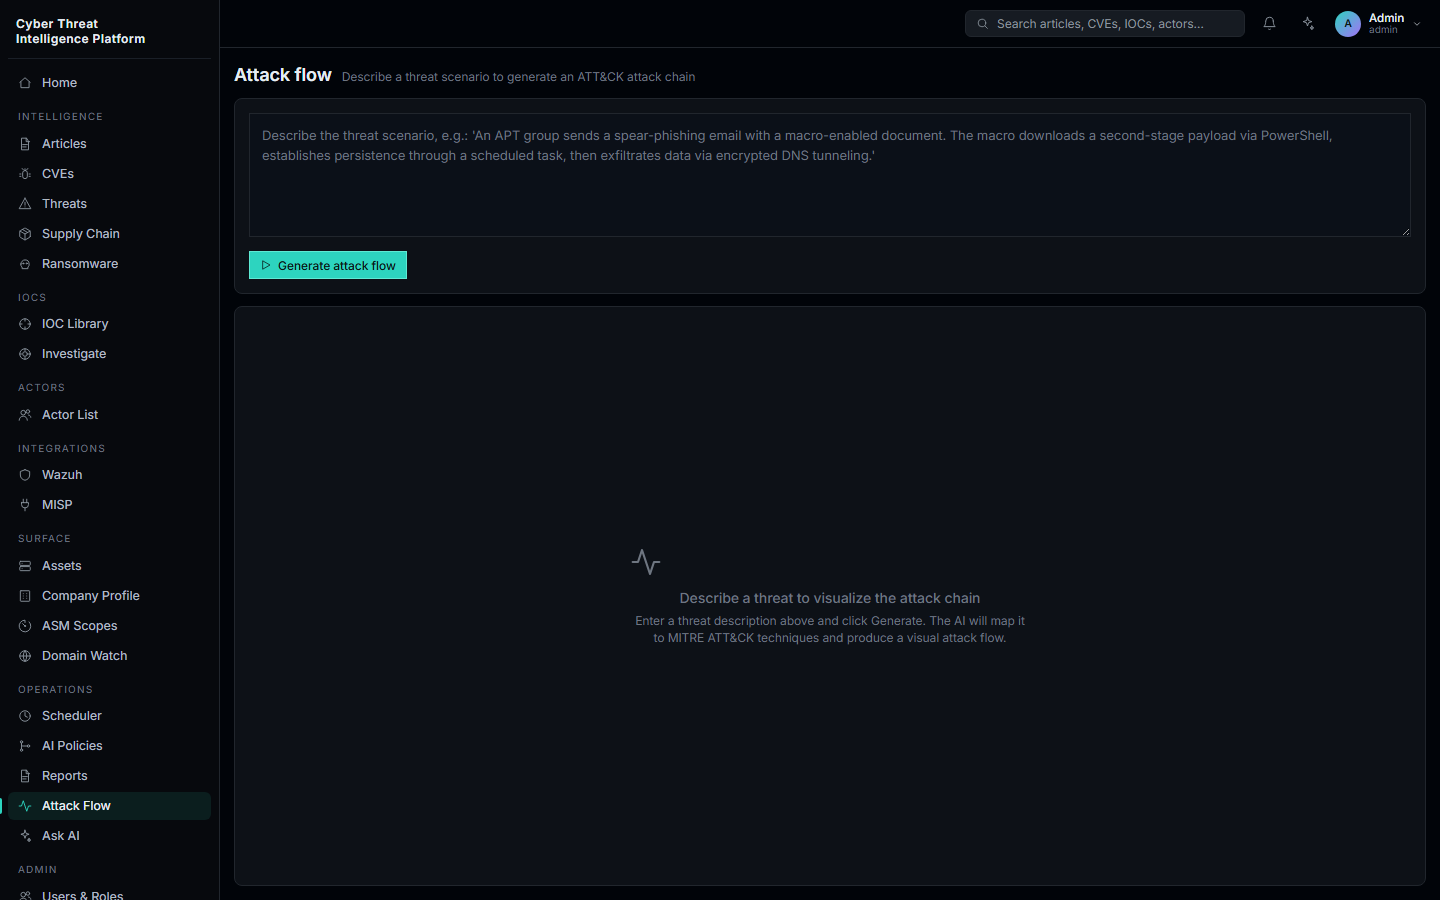
\includegraphics[width=0.95\textwidth]{images/tip/shots/33_flowviz.png}
\caption{Attack-flow visualization generated from structured analytical output.}
\label{fig:flowviz-new}
\end{figure}

\section{Containerization, Deployment, and Bootstrap}
Each service is packaged as its own image. This isolates dependencies and keeps rebuild scope bounded. The deployment topology is shown in Figures~\ref{fig:deploy-new} and \ref{fig:deploy-bottom}.

\begin{figure}[H]
\centering
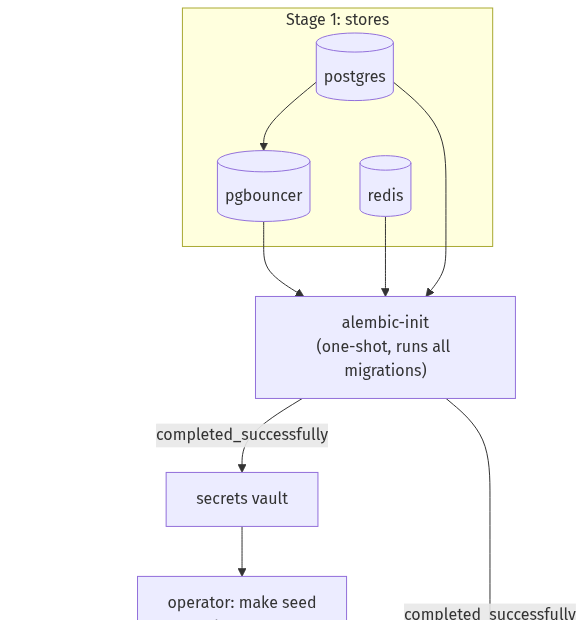
\includegraphics[width=0.72\textwidth]{images/tip/diagrams/05_deployment_topology_top.png}
\caption{Single-host deployment topology, startup and infrastructure segment.}
\label{fig:deploy-new}
\end{figure}

\begin{figure}[H]
\centering
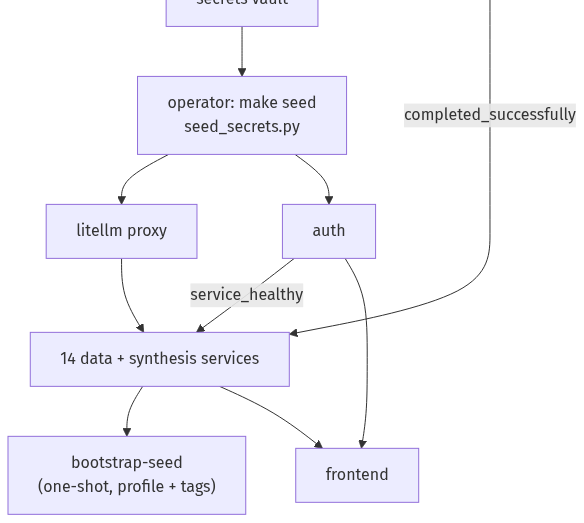
\includegraphics[width=0.72\textwidth]{images/tip/diagrams/05_deployment_topology_bottom.png}
\caption{Single-host deployment topology, service bring-up and application segment.}
\label{fig:deploy-bottom}
\end{figure}

The bootstrap sequence is intentionally ordered. Postgres, PgBouncer, and Redis start first. The one-shot migration container applies all Alembic migrations. The secrets service starts next, then auth and the LiteLLM proxy, followed by the remaining services. This ordering is enforced through Compose dependencies and health conditions rather than by manual sequencing.

This deployment choreography expresses an implicit dependency graph that exists whether it is documented or not. Databases must exist before migrations run. Secrets must exist before services can retrieve startup credentials. Authentication and key material must exist before some services can enforce request-time policy. Encoding this order explicitly in the deployment definition is an important implementation quality because it turns hidden operational knowledge into executable system behaviour.

\section{Observability, Logging, and Operator Diagnostics}
The observability model is pragmatic rather than elaborate. Each service exposes a health endpoint. Correlation IDs are propagated through middleware and bound into logs. Source-health tables show the last failure for upstream sources. Scheduler history records run state and duration. The secrets service records secret access. Together, these provide enough internal visibility for a small team to isolate common failure classes without requiring a full external telemetry stack.

Observability here should be understood as decision support for operators, not as telemetry maximalism. The goal is not to instrument every conceivable metric. The goal is to answer the kinds of questions that actually arise during failure: is the service alive, which upstream dependency is failing, which scheduled job is stuck, which secret was accessed, and which user-visible request produced the error chain in the logs. This focused notion of observability is well aligned with the platform's single-host operational model.

\section{Performance, Scalability, and Reliability}
\subsection{Performance Characteristics}
The platform is predominantly I/O bound. The main cost centres are database access, cache access, upstream feed calls, and AI inference. The most performance-sensitive path is IOC lookup, which is explicitly optimized with Redis. Other read paths favour correctness and stored-data access over aggressive caching.

\begin{figure}[H]
\centering
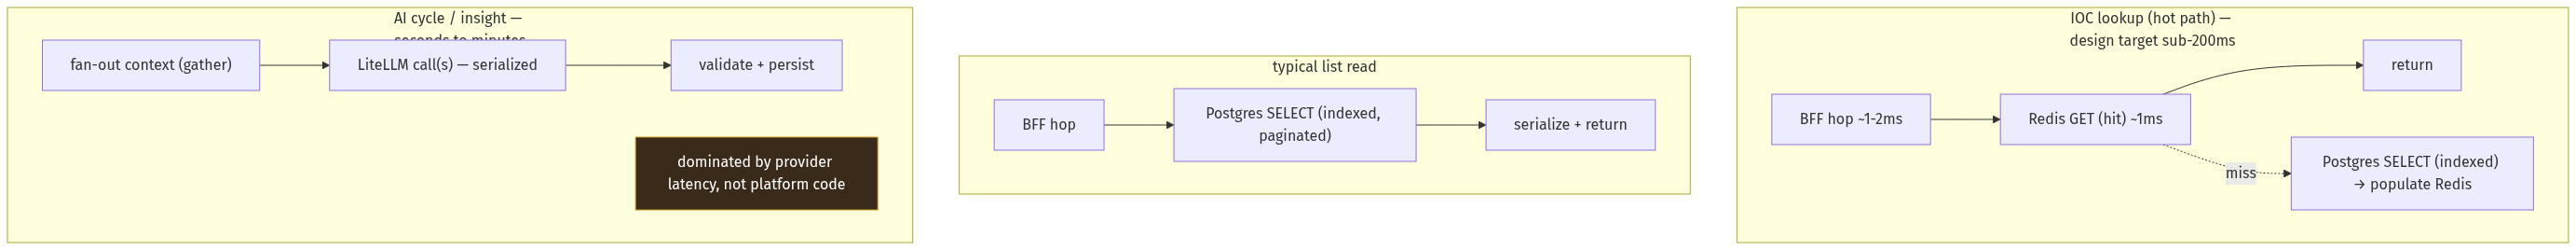
\includegraphics[width=0.9\textwidth]{images/tip/diagrams/13_latency_budget.png}
\caption{Qualitative latency budget by request class.}
\label{fig:latency-new}
\end{figure}

\subsection{Scalability Strategy}
The current deployment is single-host, but the codebase preserves several scale-friendly properties: stateless service processes, schema ownership, explicit service URLs, and isolation of AI, secrets, and scheduler concerns. Figure~\ref{fig:scaling-new} illustrates the intended scaling posture.

\begin{figure}[H]
\centering
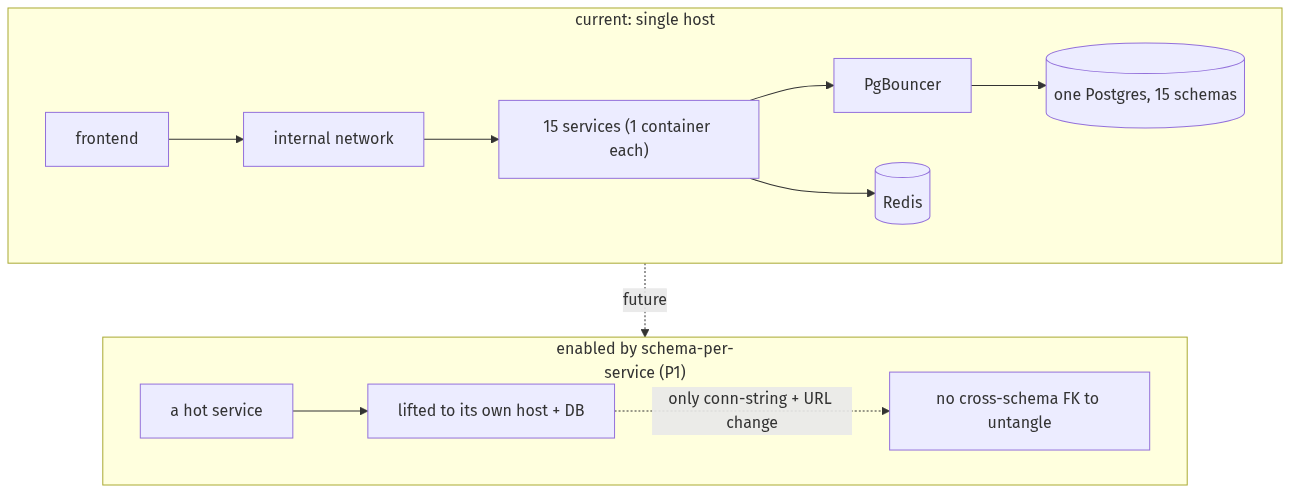
\includegraphics[width=0.9\textwidth]{images/tip/diagrams/13_scaling_model.png}
\caption{Current scaling posture and future expansion path.}
\label{fig:scaling-new}
\end{figure}

\subsection{Reliability Model}
Reliability is achieved primarily through graceful degradation, retryable source access, explicit source-health tracking, background task isolation, callback-driven scheduler semantics, and durable storage of analytical outputs. This is not a high-availability architecture in the strict sense, but it is a resilient single-host architecture.

That distinction between resilience and high availability should remain explicit. High availability concerns redundancy, failover, and continued service under infrastructure loss. Resilience concerns the ability to absorb partial dependency failure, recover predictably, and keep critical functions operating under degraded conditions. The implemented system is much stronger on the second axis than on the first, and the thesis should say so directly.

\section*{Conclusion}
\addcontentsline{toc}{section}{Conclusion}
The implementation translates architectural intent into a cohesive operating system for security analysis: consistent service construction, pooler-aware database access, resilient outbound HTTP, bounded AI integration, a real scheduler control plane, and an operator-facing interface that exposes the results. The strongest engineering choices are the separation of ingestion from synthesis, the disciplined use of shared packages, and the refusal to let AI sit on the platform's critical ingestion path. The next chapter addresses how this system is validated, where its testing posture is strong, where it is weak, and what limits remain.
